\documentclass[border=12pt]{standalone}
\usepackage[utf8]{inputenc}
\usepackage{amsmath}
\usepackage{tikz}
\usetikzlibrary{arrows.meta, positioning, calc, shapes.geometric, backgrounds, fit}

\definecolor{cloudblue}{RGB}{24, 144, 255}
\definecolor{servergray}{RGB}{45, 52, 54}
\definecolor{espgreen}{RGB}{39, 174, 96}
\definecolor{supagreen}{RGB}{62, 207, 142}
\definecolor{ngrokblue}{RGB}{31, 80, 163}
\definecolor{rblue}{RGB}{39, 109, 195}
\definecolor{cardbg}{RGB}{248, 250, 252}

\begin{document}
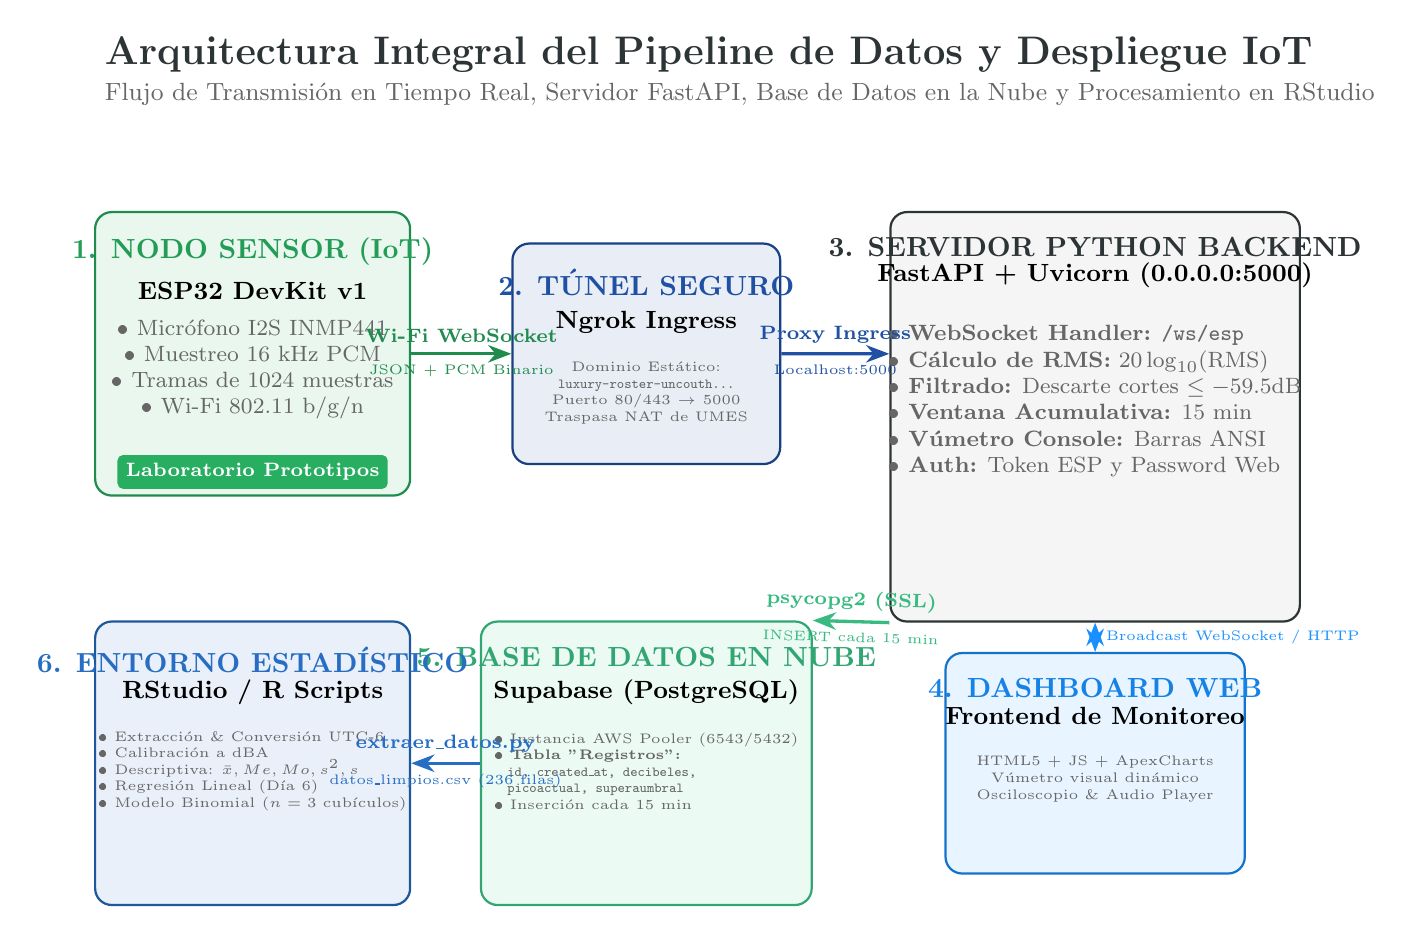
\begin{tikzpicture}[font=\sffamily, scale=1.0, >=Stealth]

    % =========================================================================
    % TÍTULO DEL DIAGRAMA
    % =========================================================================
    \node[anchor=west, font=\bfseries\Large, text=servergray] at (-0.5, 9.8) {Arquitectura Integral del Pipeline de Datos y Despliegue IoT};
    \node[anchor=west, font=\small, text=gray!80!black] at (-0.5, 9.3) {Flujo de Transmisión en Tiempo Real, Servidor FastAPI, Base de Datos en la Nube y Procesamiento en RStudio};

    % =========================================================================
    % BLOQUE 1: NODO IoT (ESP32 + INMP441)
    % =========================================================================
    \node[draw=espgreen!80!black, fill=espgreen!10, thick, rounded corners=6pt, minimum width=4.0cm, minimum height=3.6cm, align=center] (ESP) at (1.5, 6.0) {};
    \node[font=\bfseries\normalsize, text=espgreen!90!black, anchor=north] at (1.5, 7.6) {1. NODO SENSOR (IoT)};
    \node[font=\small\bfseries, text=black] at (1.5, 6.8) {ESP32 DevKit v1};
    \node[font=\footnotesize, text=gray!80!black, align=center] at (1.5, 5.8) {
        • Micrófono I2S INMP441\\
        • Muestreo $16\text{ kHz}$ PCM\\
        • Tramas de 1024 muestras\\
        • Wi-Fi 802.11 b/g/n
    };
    \node[fill=espgreen, text=white, font=\scriptsize\bfseries, rounded corners=2pt, inner sep=3pt] at (1.5, 4.5) {Laboratorio Prototipos};

    % =========================================================================
    % BLOQUE 2: TÚNEL NGROK (EXPOSICIÓN GLOBAL)
    % =========================================================================
    \node[draw=ngrokblue!80!black, fill=ngrokblue!10, thick, rounded corners=6pt, minimum width=3.4cm, minimum height=2.8cm, align=center] (NGROK) at (6.5, 6.0) {};
    \node[font=\bfseries\normalsize, text=ngrokblue, anchor=north] at (6.5, 7.2) {2. TÚNEL SEGURO};
    \node[font=\small\bfseries, text=black] at (6.5, 6.4) {Ngrok Ingress};
    \node[font=\tiny, text=gray!80!black, align=center] at (6.5, 5.5) {
        Dominio Estático:\\
        \texttt{luxury-roster-uncouth...}\\
        Puerto 80/443 $\rightarrow$ 5000\\
        Traspasa NAT de UMES
    };

    % =========================================================================
    % BLOQUE 3: SERVIDOR UBUNTU / FASTAPI (NUBE)
    % =========================================================================
    \node[draw=servergray, fill=gray!8, thick, rounded corners=6pt, minimum width=5.2cm, minimum height=5.2cm, align=center] (SRV) at (12.2, 5.2) {};
    \node[font=\bfseries\normalsize, text=servergray, anchor=north] at (12.2, 7.6) {3. SERVIDOR PYTHON BACKEND};
    \node[font=\small\bfseries, text=black] at (12.2, 7.0) {FastAPI + Uvicorn (0.0.0.0:5000)};
    \node[font=\footnotesize, text=gray!80!black, align=left] at (12.2, 5.4) {
        • \textbf{WebSocket Handler:} \texttt{/ws/esp}\\
        • \textbf{Cálculo de RMS:} $20\log_{10}(\text{RMS})$\\
        • \textbf{Filtrado:} Descarte cortes $\le -59.5\text{dB}$\\
        • \textbf{Ventana Acumulativa:} 15 min\\
        • \textbf{Vúmetro Console:} Barras ANSI\\
        • \textbf{Auth:} Token ESP y Password Web
    };

    % =========================================================================
    % BLOQUE 4: FRONTEND WEB DE MONITOREO
    % =========================================================================
    \node[draw=cloudblue!80!black, fill=cloudblue!10, thick, rounded corners=6pt, minimum width=3.8cm, minimum height=2.8cm, align=center] (FRONT) at (12.2, 0.8) {};
    \node[font=\bfseries\normalsize, text=cloudblue!90!black, anchor=north] at (12.2, 2.0) {4. DASHBOARD WEB};
    \node[font=\small\bfseries, text=black] at (12.2, 1.4) {Frontend de Monitoreo};
    \node[font=\tiny, text=gray!80!black, align=center] at (12.2, 0.6) {
        HTML5 + JS + ApexCharts\\
        Vúmetro visual dinámico\\
        Osciloscopio \& Audio Player
    };

    % =========================================================================
    % BLOQUE 5: BASE DE DATOS SUPABASE (POSTGRESQL NUBE)
    % =========================================================================
    \node[draw=supagreen!80!black, fill=supagreen!10, thick, rounded corners=6pt, minimum width=4.2cm, minimum height=3.6cm, align=center] (SUPA) at (6.5, 0.8) {};
    \node[font=\bfseries\normalsize, text=supagreen!80!black, anchor=north] at (6.5, 2.4) {5. BASE DE DATOS EN NUBE};
    \node[font=\small\bfseries, text=black] at (6.5, 1.7) {Supabase (PostgreSQL)};
    \node[font=\tiny, text=gray!80!black, align=left] at (6.5, 0.7) {
        • Instancia AWS Pooler (6543/5432)\\
        • \textbf{Tabla "Registros":}\\
        \ \ \texttt{id, created\_at, decibeles,}\\
        \ \ \texttt{picoactual, superaumbral}\\
        • Inserción cada 15 min
    };

    % =========================================================================
    % BLOQUE 6: COMPUTACIÓN ESTADÍSTICA (RSTUDIO)
    % =========================================================================
    \node[draw=rblue!80!black, fill=rblue!10, thick, rounded corners=6pt, minimum width=4.0cm, minimum height=3.6cm, align=center] (RSTUDIO) at (1.5, 0.8) {};
    \node[font=\bfseries\normalsize, text=rblue, anchor=north] at (1.5, 2.4) {6. ENTORNO ESTADÍSTICO};
    \node[font=\small\bfseries, text=black] at (1.5, 1.7) {RStudio / R Scripts};
    \node[font=\tiny, text=gray!80!black, align=left] at (1.5, 0.7) {
        • Extracción \& Conversión UTC-6\\
        • Calibración a $\text{dBA}$\\
        • Descriptiva: $\bar{x}, Me, Mo, s^2, s$\\
        • Regresión Lineal (Día 6)\\
        • Modelo Binomial ($n=3$ cubículos)
    };

    % =========================================================================
    % LÍNEAS DE CONEXIÓN Y FLUJO DE DATOS
    % =========================================================================
    % ESP32 -> NGROK
    \draw[->, very thick, espgreen!80!black] (ESP.east) -- (NGROK.west)
        node[midway, above, font=\scriptsize\bfseries] {Wi-Fi WebSocket}
        node[midway, below, font=\tiny] {JSON + PCM Binario};

    % NGROK -> FASTAPI
    \draw[->, very thick, ngrokblue] (NGROK.east) -- ($(SRV.west)+(0, 0.8)$)
        node[midway, above, font=\scriptsize\bfseries] {Proxy Ingress}
        node[midway, below, font=\tiny] {Localhost:5000};

    % FASTAPI <-> FRONTEND
    \draw[<->, very thick, cloudblue] (SRV.south) -- (FRONT.north)
        node[midway, right, font=\tiny] {Broadcast WebSocket / HTTP};

    % FASTAPI -> SUPABASE
    \draw[->, very thick, supagreen!90!black] (SRV.south west) -- (SUPA.north east)
        node[midway, above, sloped, font=\scriptsize\bfseries] {psycopg2 (SSL)}
        node[midway, below, sloped, font=\tiny] {INSERT cada 15 min};

    % SUPABASE -> RSTUDIO
    \draw[->, very thick, rblue] (SUPA.west) -- (RSTUDIO.east)
        node[midway, above, font=\scriptsize\bfseries] {extraer\_datos.py}
        node[midway, below, font=\tiny] {datos\_limpios.csv (236 filas)};

\end{tikzpicture}
\end{document}
